\chapter{Introduction}\label{ch:introduction}
\emph{Pad-fs} (Piattaforme Abilitanti Distribuite - File System) is a distributed file system that store key value pairs. It is written in \textit{Java}  and uses \textit{Apache Maven} for the project management. The git version can be found \url{https://github.com/dido18/PAD-FileSystem}.

A high level overview of the \emph{Pad-fs} system architecture is shown in figure~\ref{fig:architecture}. It is composed by two parts: the \textit{storage system} and the \textit{client} node.
\begin{figure}
\centering
\includegraphics[scale=0.5]{figures/architecture.png}
\caption{Pad-fs architecture overview}
\label{fig:architecture}
\end{figure}

\begin{itemize}
\item The \textbf{storage system} is a set of communicating storage nodes that are responsible to manage the data to be stored. 
Each storage node has a local database and it is composed by two main services:
\begin{itemize}
\item \textit{GossipService} is a background thread that perform the gossiping protocol.
\item \textit{StorageService} is the service that listen for incoming messages on storage port and performs the operation on the persistent storage (add values, remove values, update versions, resolve conflict, quorum system, etc...).
\end{itemize}

\item The \textbf{client} is an external independent node that interact with the storage system in order to perform the file system operations. An user interacts with  the client through a \textit{cli}. The client, upon an user input operation, determines the master node, constructs the proper message and send it to the master node selected. In order to know the master node of a key, the client has the same consistent hashing logic of the storage system. Client exposes four API operations to the user: get, put, list, rm.

The client node  has two main modules:
\begin{itemize}
\item   \textit{Cli} (command line interface) receives user's inputs and sends messages to the storage system.
\item \textit{Client Gossip}  keeps updated the client's view of the storage system system. It asks periodically to a random node in the storage system the current active nodes.
\end{itemize}

\item \textbf{User} is who submit the operation into the system through the cli.
\end{itemize}

